%   Include in problem formulation
%   target 2p 
\autsection{Communications for Europa}{Gustavo Feijóo Carrillo}
%   Introductory paragraph
%   Mission Stages and necessary comm links
%       Interplanetary phase

%--> False ref handling
%\iffalse
%(seen on fig. \ref{fig:GalInst1} and \ref{fig:GalInst2})
%\fi

A mission to Europa would be classified as an interplanetary mission, furthermore this one is much more than just that and requires careful considerations of the different scenarios that a mission for Europa's sub-ice ocean exploration requires. First, the interplanetary phase is considered from launch of the spacecraft until Jupiter's orbit insertion (JOI). Second, is the landing phase just after accomplishing EOI (Europa Orbit Insertion), where site determination and certification procedures are carried before the landing of the carrier itself. Third (and most importantly for this writing) is the penetrator release and its descent through the ice crust which requires new development for accomplishing a working communications link through several kilometers of ice. And, at this phase is where the main scientific objectives are to be carried out as well as the majority of all the mission's goals.

\begin{figure}[htb]
	\centering
	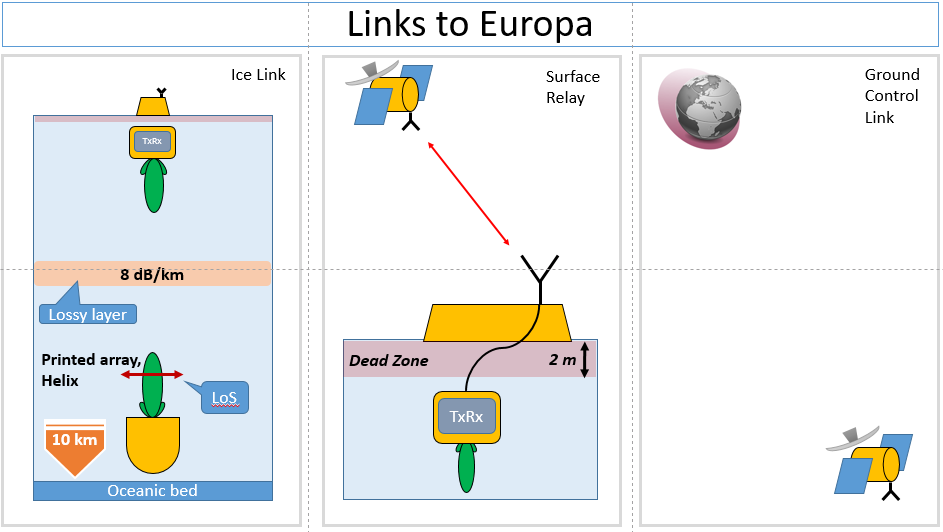
\includegraphics[width=\textwidth]{figures/comms/europaLinks}
	\caption{ \textit{DRAFT} Depiction of the three main stages of a mission to Europa from a telecommunications perspective.}
	\label{fig:europaLinks}
\end{figure}

The interplanetary link is feasible thanks to the development of deep space communication networks by ESA (ESTRACK) and NASA (DSN), increasing the reliability of communications and navigation of spacecrafts on missions beyond Earth's orbit. This makes the main hazard during this phase, the high radiation environment of interplanetary space which requires designing for single fault tolerance, a redundant transponder system would be the must straight forward approach. Other problem for this mission stage is the pointing of the antennas since the higher gains needed, increase the requirements for the attitude control systems to keep direct line of sight with ground tracking stations. Universal Space Transponders (UST) are available for down/up-link in UHF with proven capabilities from previous missions to Mars with the inclusion of a down/up-link at X-band and a Ka-band down-link (UHF is TRL-9 and X,Ka-band is TRL-4 according to \cite{clipper}). This leads to focus on the details of a link with a possible Europa orbiter and more important the communications through the ice crust between the penetrator and the lander. After reaching the Jovian system, the most critical communication situation is for landing site determination and landing maneuvers as the propagation delay of 1 hour and 46 minutes makes only an autonomous solution possible which will need the highest data link coherence, robustness and concurrency.

The problem of establishing communications between the penetrator and the lander for command and telemetry as well as scientific data download is the propagation medium. The Europan ice crust is yet to be fully characterized, most models rely on data from 2 to 4 flybys from the Galileo mission and have developed models for the crust behaviour and composition as found in \cite{Chyba}. The ice losses aren't an issue itself since it has been well established through empirical work and modeling, as found in \cite{iceLink-scott}. Liquid water is considered opaque at radio- and micro-wave frequencies but in frozen state, water ice shows a very low imaginary dielectric constant which dictates the level of intensity loss of an electromagnetic plane wave traveling through this medium, this constant $\epsilon''$ is about a thousand times smaller than for liquid water. This fact allows for the possibility of an ice based communications link. In the following chapters a more detailed section on how the ice losses are expected to be found at Europa will be exposed. This detailed section will include a discussion on the effect of salt contents in the ice and its effect on the propagation loss. Similarly, the effect of different ice temperature must be discussed since it has a major contribution on the propagation loss of this medium. A link able to cope with this propagation losses is what will allow the penetrator to melt through several kilometers of ice and complete the mission objectives following the ice crust depth at the landing site is conisdered unknown, spanning from a few thousand meters $(3-5 km)$ to a thick crust close to $20 km$ wide.

Other problem for the penetrator-lander link is the the liquid water and "slushy" ice surrounding the penetrator vessel, a good understanding of the melt-refreeze cycle must be reached in order to achieve a robust communications link. Previous studies carried out by JPL for a similar mission requiring a through ice link assumed the refreezing without any details \cite{iceLink-scott}, for this mission this assumption is not good enough and must seek deeper understanding as stated before. 

\begin{figure}[htb]
	\centering
	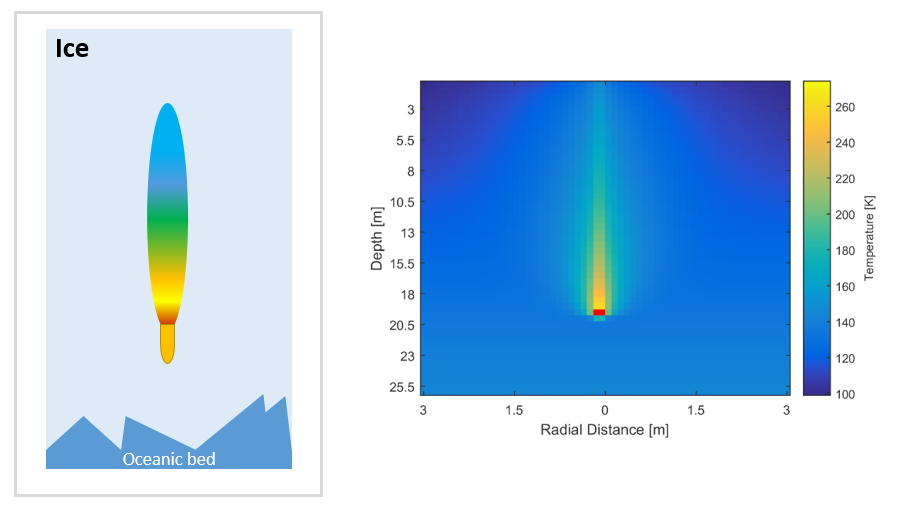
\includegraphics[width=\textwidth]{figures/comms/meltColCycle_0}
	\caption{ \textit{DRAFT} Depiction of the plausible melted water column forming behind the penetrator with possible adverse effect on the performance of the communications from penetrator to lander. This column could be as short as 4 m or reach a few tens of meters.}
	\label{fig:meltColumn_broad}
\end{figure}
